%!TEX root = pixel-wise-street-segmentation.tex

\section{Evaluation}\label{sec:evaluation}

In the following section we will discuss the results of our approach. First, we will compare our different approaches with each other and then finally we will compare our best approach to stanfrodpaper work (which is ranked on place 1 at KITTI road segmentation).
As already stated, the KITTI Road Estimation dataset the basis for our evaluation.

When we were conducting the first steps of our evaluation we only worked on the training data of the KITTI data set.

As the ground truth is only given for the training data set we split it 20 to 80(test/training)in order to be able to measure our performance. SO we compareds
Finally we used the KITTI official evaluation side [link to webside].

Working with our neural networks we realised that there are a lot of parameters which need to be taken care of. Firstly we evaluated different once considering run time and performance.
On the one hand we have parameters not really affecting the neural network, like patch size, different image size(training testing) and on the other side we have filter-size number of neural layers and so on.
So based on this we figured out the best combination on our training set and then handed it in the KITTI evaluation.

In the following we will have a more precise look at the parameters and results of our neural networks.

For the following evaluation we used a computer with:
\begin{itemize}
\item Intel(R) Core(TM) i7-4790K CPU @ 4.00GHz
\item System memory 16 GiB
\item GeForce GTX 980 4GiB Ram
\end{itemize}

Runtime
      \begin{table}[h!]
  \begin{center}
    \begin{tabular}{c|ccc}
    \toprule
      \textbf{Netztyp/Stride} & \textbf{10} & \textbf{37} & \textbf{51} \\
     \midrule
      \textbf{Regression} & 1.99 & 0.29 & 0.18 \\
      \textbf{Klassifikation} & 1.83 & 0.2 & 0.11\\
      \bottomrule
    \end{tabular}
        \caption{Ausf\"uhrungszeit pro Bild (621x188 Pixel) in Sekunden.}
  \end{center}
\end{table}

perfomance
      \begin{table}[h!]
  \begin{center}
   % \caption{Caption for the table.}
    \label{tab:table1}
    \begin{tabular}{c|ccccc}
    \toprule
      \textbf{Netztyp} & \textbf{TN} & \textbf{FP} & \textbf{FN} & \textbf{TP} & \textbf{ACC} \\
       \midrule
      \textbf{Reg. - Stride 10} & 0.977 & 0.022 & 0.197 & 0.802 & 0.947\\
      \textbf{Reg. - Stride 37} & 0.973 & 0.026 & 0.176 & 0.823 &  \textcolor{red}{0.948}\\ 
      \textbf{Reg. - Stride 51} & 0.969 & 0.030 & 0.165 & \textcolor{red}{0.834} & 0.946\\
      \midrule
      \textbf{Kla. - Stride 10} & 0.981 & 0.018 & 0.241 & 0.758 & 0.942\\
      \textbf{Kla. - Stride 37} & 0.959 & 0.040 & 0.212 & 0.787 & 0.929\\
      \textbf{Kla. - Stride 51} & \textcolor{red}{0.982} & 0.017 & 0.451 & 0.548 & 0.906\\
      \bottomrule
    \end{tabular}
    \caption{Ergebnisse der verschiedene neuronalen Netze auf Testset (58 Bilder, ~ 6,7 Mil. Pixel)}
  \end{center}
\end{table}

\textbf{kitti performance!!!!!!!!!!!!!!!!!!!!!!!!!!!!!!!!}
In the following we will look more closely at our results and differ between the different road types (UM, UMM, UU, URBAN).

      \begin{table}[h!]
  \begin{center}
\begin{tabular}{c | c | c | c | c | c | c}
 {\bf Benchmark} & {\bf MaxF} & {\bf AP} & {\bf PRE} & {\bf REC} & {\bf FPR} & {\bf FNR}\\ \hline
UM\_ROAD & 67.91 \% & 61.63 \% & 86.90 \% & 55.74 \% & 3.83 \% & 44.26 \%\\
UMM\_ROAD & 79.67 \% & 78.41 \% & 93.29 \% & 69.51 \% & 5.50 \% & 30.49 \%\\
UU\_ROAD & 56.48 \% & 51.89 \% & 84.67 \% & 42.37 \% & 2.50 \% & 57.63 \%\\
URBAN\_ROAD & 71.10 \% & 65.14 \% & 89.83 \% & 58.84 \% & 3.67 \% & 41.16 \%\\
\end{tabular}
  \end{center}
\end{table}

Here, red denotes false negatives, blue areas correspond to false positives and green represents true positives. 

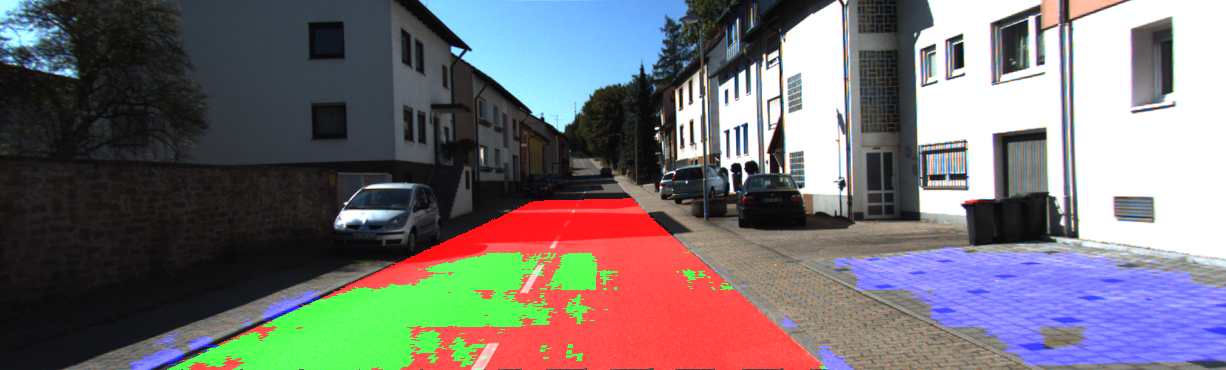
\includegraphics[scale=0.2]{figures/kitty_eval/Persp_um_road_000077.png}
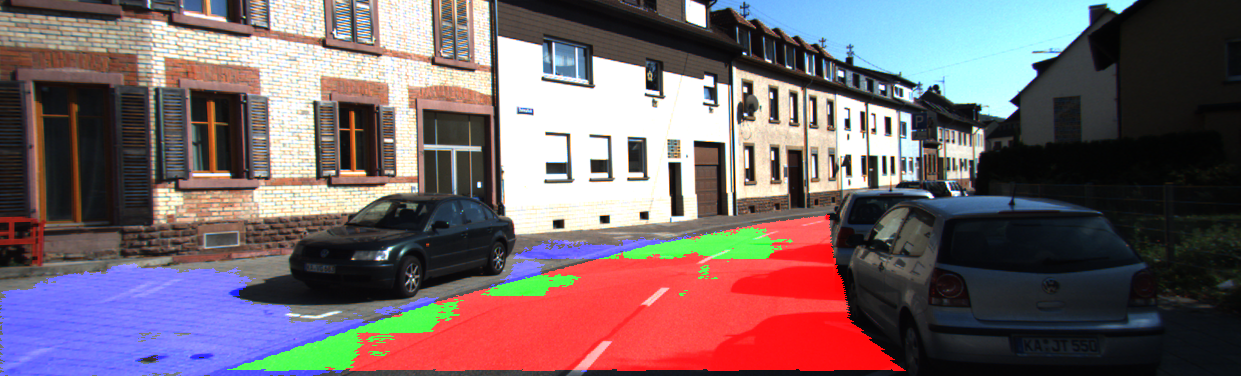
\includegraphics[scale=0.2]{figures/kitty_eval/Persp_um_road_000095.png}
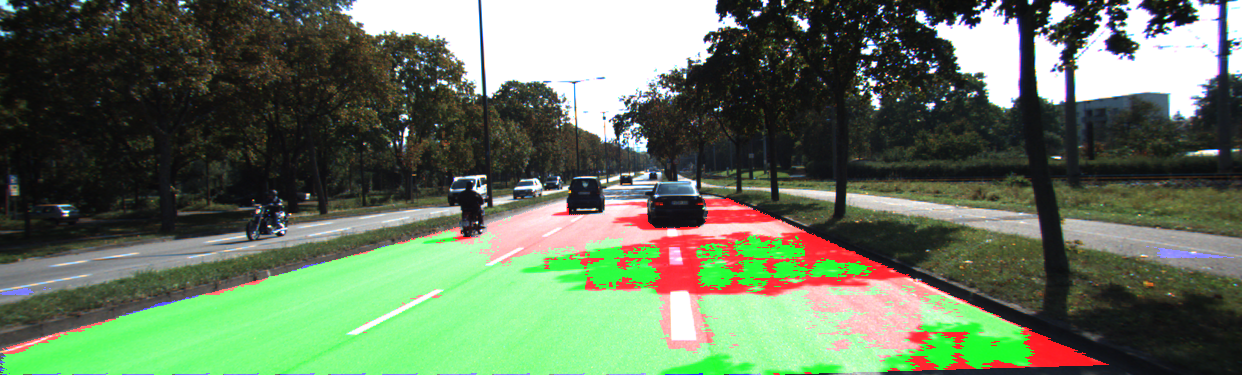
\includegraphics[scale=0.2]{figures/kitty_eval/Persp_umm_road_000025.png}
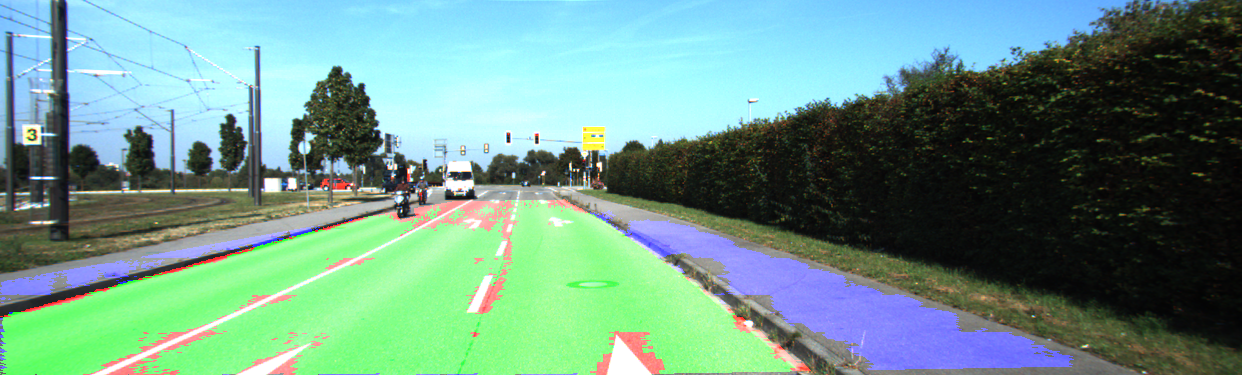
\includegraphics[scale=0.2]{figures/kitty_eval/Persp_umm_road_000040.png}
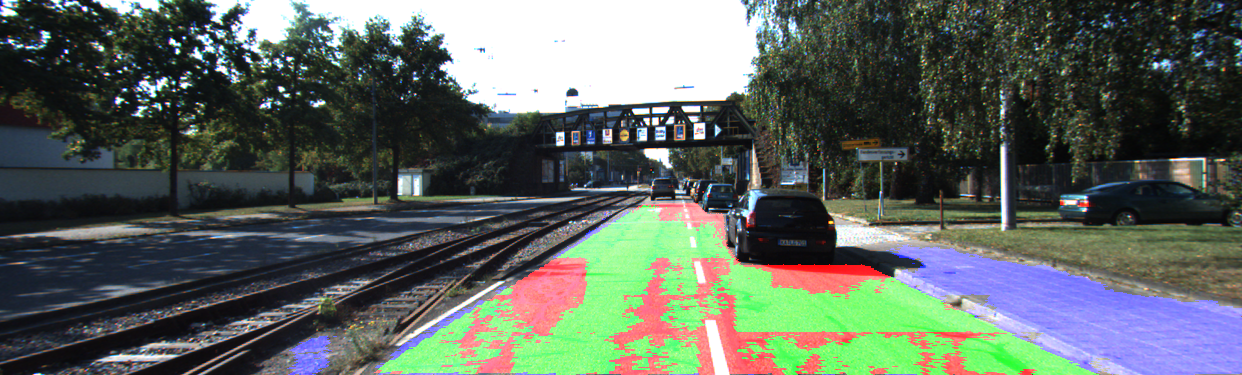
\includegraphics[scale=0.2]{figures/kitty_eval/Persp_umm_road_000066.png}
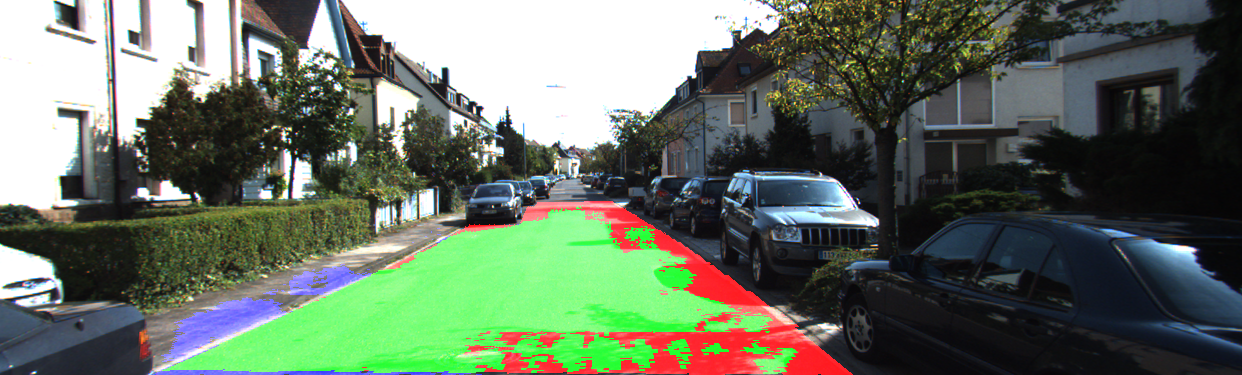
\includegraphics[scale=0.2]{figures/kitty_eval/Persp_uu_road_000020.png}
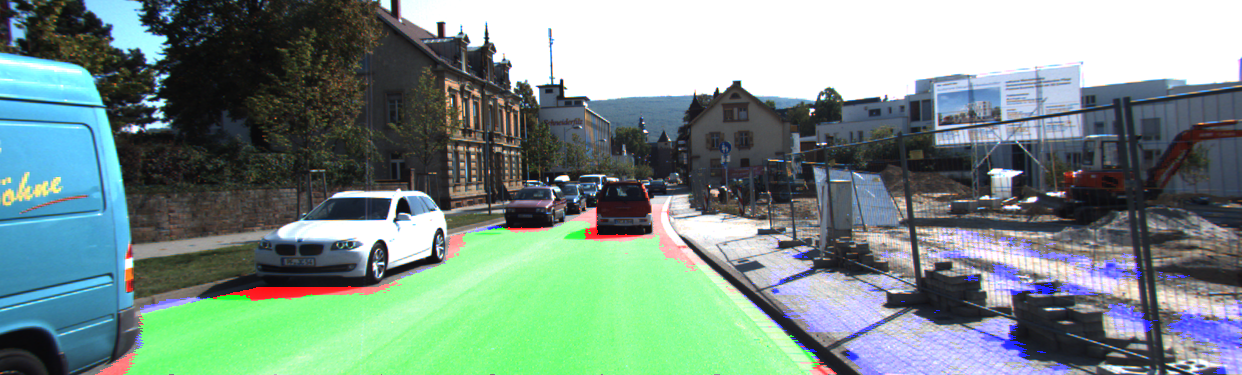
\includegraphics[scale=0.2]{figures/kitty_eval/Persp_uu_road_000027.png}
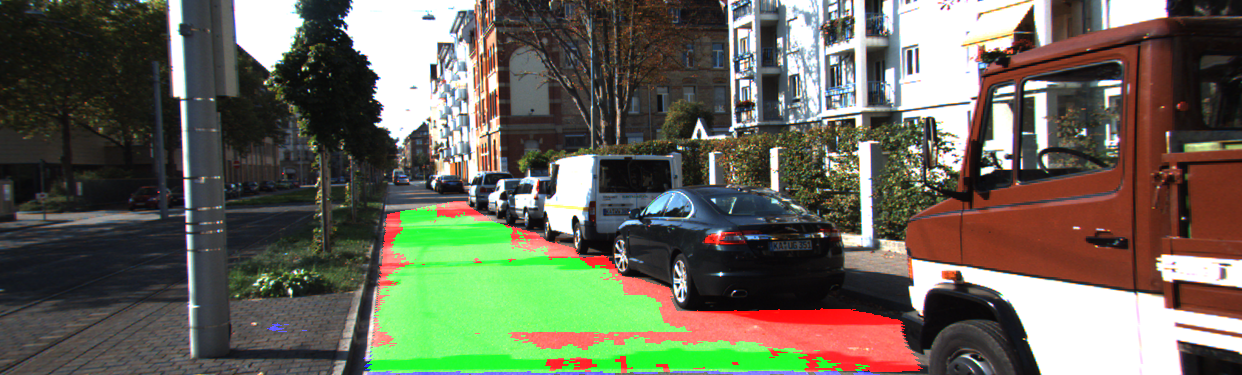
\includegraphics[scale=0.2]{figures/kitty_eval/Persp_uu_road_000082.png}



%Unfortunately the ram of the graphic card limited our possibility to use larger patch sizes.
